\documentclass[8pt,a4paper,compress]{beamer}

\usepackage{/home/siyer/lib/slides}

\title{Lexical Analysis}
\date{}

\begin{document}
\begin{frame}
\vfill
\titlepage
\end{frame}

\begin{frame}
\frametitle{Outline}
\tableofcontents
\end{frame}

\section{Scanning Tokens}
\begin{frame}[fragile]
\pause

The first step in compiling a program is to break it into tokens (aka lexemes); for example, given the \jmm program

\begin{lstlisting}[language=Java]
package pass;

import java.lang.System;

public class Factorial {
    // Two methods and a field
    public static int factorial(int n) {
        if (n <= 0)
            return 1;
        else
            return n * factorial(n - 1);
    }
    
    public static void main(String[] args) {
        int x = n;
        System.out.println(x + "! = " + factorial(x));
    }

    static int n = 5;
}
\end{lstlisting}

we want to produce the sequence of tokens \lstinline{package}, \lstinline{pass}, \lstinline{;},\lstinline{import}, \lstinline{java}, \lstinline{.}, \lstinline{lang}, \lstinline{.}, \lstinline{System},\lstinline{;}, \lstinline{public},\lstinline{class}, \lstinline{Factorial}, \lstinline${$,\lstinline{public}, \lstinline{static}, \lstinline{int},\lstinline{factorial}, \lstinline{(},\lstinline{int}, \lstinline{n,)}, \lstinline${$, \lstinline{if}, \lstinline{(}, \lstinline{n},\lstinline{<=}, \lstinline{0}, \lstinline{)}, \lstinline$}$, \lstinline{return}, \lstinline{1},\lstinline{;}, \lstinline{else},\lstinline{return}, \lstinline{n}, \lstinline{*}, \lstinline{factorial}, \lstinline{(}, \lstinline{n}, \lstinline{-}, \lstinline{1}, \lstinline{)}, \lstinline$}$, \lstinline{;}, \lstinline$}$, \lstinline{public}, \lstinline{static}, \lstinline{void}, \lstinline{main}, \lstinline{(}, \lstinline{String}, \lstinline{[}, \lstinline{]}, \lstinline{args}, \lstinline{)}, \lstinline$}$, \lstinline${$, \lstinline{int}, \lstinline{x}, \lstinline{=}, \lstinline{n}, \lstinline{;}, \lstinline{System}, \lstinline{.}, \lstinline{out}, \lstinline{.}, \lstinline{println}, \lstinline{(}, \lstinline{x}, \lstinline{+}, \lstinline{"!="}, \lstinline{+}, \lstinline{factorial}, \lstinline{(}, \lstinline{x}, \lstinline{)}, \lstinline{)}, \lstinline$}$, \lstinline{;}, \lstinline$}$, \lstinline{static}, \lstinline{int}, \lstinline{n}, \lstinline{=}, \lstinline{5},\lstinline{;}, and \lstinline$}$

\end{frame}

\begin{frame}[fragile]
\pause

We separate the lexemes into categories; in our example program
\begin{itemize}
\item \lstinline{public}, \lstinline{class}, \lstinline{static}, and \lstinline{void} are reserved words

\item \lstinline{Factorial}, \lstinline{main}, \lstinline{String}, \lstinline{args}, \lstinline{System}, \lstinline{out}, and \lstinline{println} are all identifiers

\item The string \lstinline{!=} is a literal, a string literal in this instance

\item The rest are operators and separators
\end{itemize}

\pause
\bigskip

The program that breaks the input stream of characters into tokens is called a lexical analyzer or a scanner

\pause
\bigskip

A scanner may be hand-crafted or it may be generated automatically from a specification consisting of a sequence of regular expressions

\pause
\bigskip

A state transition diagram is a natural way of describing a scanner
\end{frame}

\begin{frame}[fragile]
\pause

A state transition diagram for identifiers and integers and the corresponding code
\begin{center}
\visible<2->{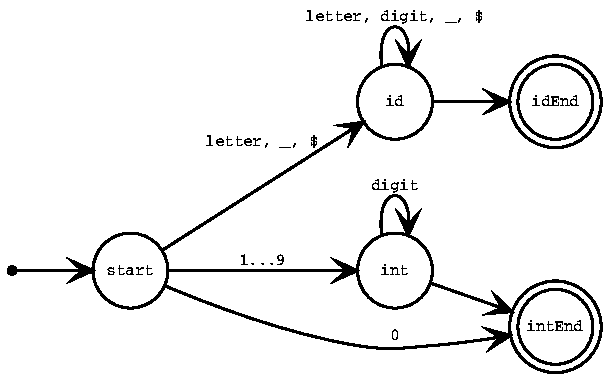
\includegraphics[scale=0.6]{{figures/figure02.01}.jpg}}
\end{center}

\begin{lstlisting}[language=Java]
    if (isLetter(ch) || ch == '_' || ch == '$') {
        buffer = new StringBuffer();
        while (isLetter(ch) || isDigit(ch) || ch == '_' || ch == '$'){
            buffer.append(ch);
            nextCh();
        }
        return new TokenInfo(IDENTIFIER, buffer.toString(), line);
    }
\end{lstlisting}
\end{frame}

\begin{frame}[fragile]
\pause

\begin{lstlisting}[language=Java]
    else if (ch == '0') {
        nextCh();
        return new TokenInfo(INT_LITERAL, "0", line);
    }
    else if (isDigit(ch)){
        buffer = new StringBuffer();
        while (isDigit(ch)) {
            buffer.append(ch);
            nextCh();
        }
        return new TokenInfo(INT_LITERAL, buffer.toString(), line);
    }
\end{lstlisting}
\end{frame}

\begin{frame}[fragile]
\pause

A state transition diagram for reserved words and the corresponding code
\begin{center}
\visible<2->{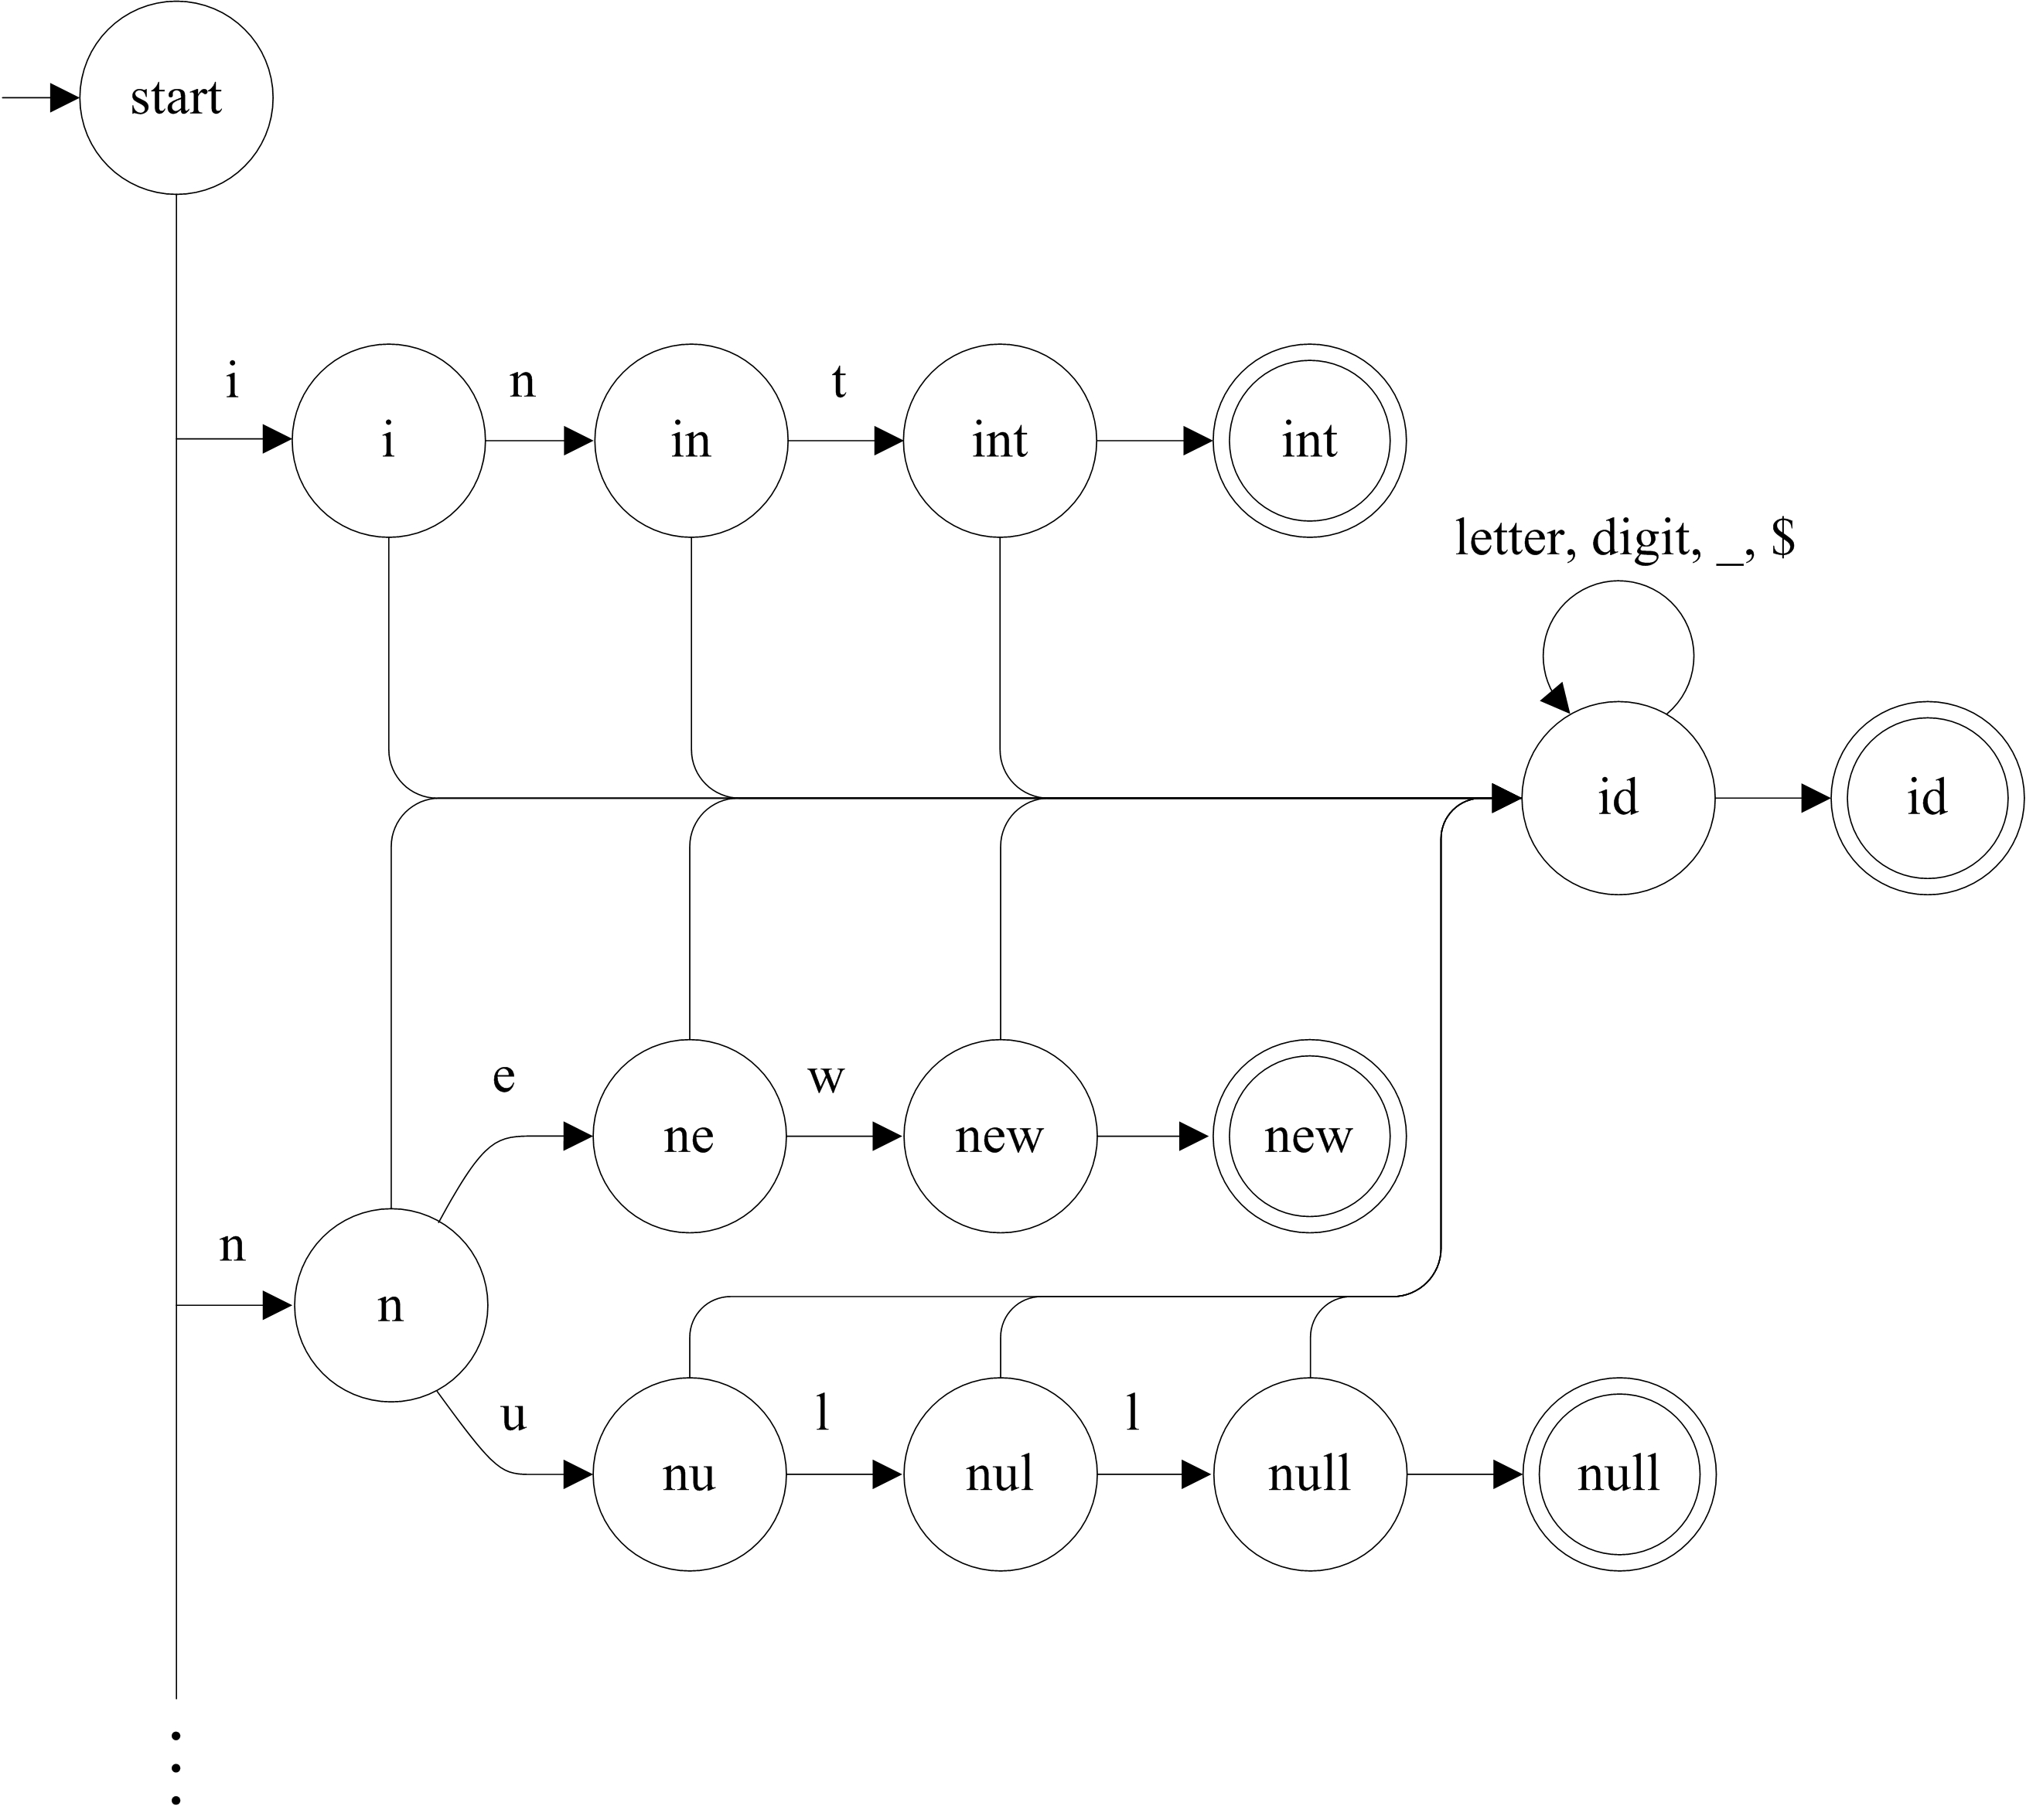
\includegraphics[scale=0.6]{{figures/figure02.02}.jpg}}
\end{center}
\end{frame}

\begin{frame}[fragile]
\pause

\begin{lstlisting}[language=Java]
...
else if (ch == 'n') {
    buffer.append(ch);
    nextCh();
    if (ch == 'e') {
        buffer.append(ch);
        nextCh();
        if (ch == 'w') {
            buffer.append(ch);
            nextCh();
            if (!isLetter(ch) && !isDigit(ch) && ch != '_' && ch !=  '$') {
                return new TokenInfo(NEW, line);
            }
        }
    }
    else if (ch == 'u') {
        buffer.append(ch);
        nextCh();
        if (ch == 'l') {
            buffer.append(ch);
            nextCh();
            if (ch == 'l') {
                buffer.append(ch);
                nextCh();
                if (!isLetter(ch) && !isDigit(ch) && ch != '_' && ch !=  '$') {
                    return new TokenInfo(NULL, line);
                }
            }
        }
    }
\end{lstlisting}
\end{frame}

\begin{frame}[fragile]
\pause

\begin{lstlisting}[language=Java]
    while (isLetter(ch) || isDigit(ch) || 
            ch == '_' || ch == '$') {
        buffer.append(ch);
        nextCh();
    }
    return new TokenInfo(IDENTIFIER, buffer.toString(), line);
}
else ...
\end{lstlisting}

\pause
\bigskip

A better approach for recognizing reserved words
\begin{center}
\visible<3->{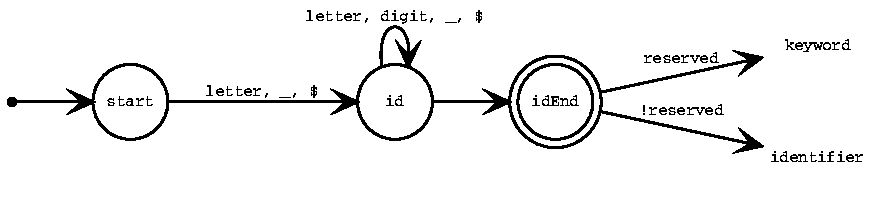
\includegraphics[scale=0.6]{{figures/figure02.03}.jpg}}
\end{center}
\end{frame}

\begin{frame}[fragile]
\pause

\begin{lstlisting}[language=Java]
    if (isLetter(ch) || ch == '_' || ch == '$') {
        buffer = new StringBuffer();
        while (isLetter(ch) || isDigit(ch) || 
               ch == '_' || ch == '$'){
            buffer.append(ch);
            nextCh();
        }
        String identifier = buffer.toString();                 
        if (reserved.containsKey(identifier)) {
            return new TokenInfo(reserved.get(identifier), line); 
        }
        else {                     
            return new TokenInfo(IDENTIFIER, identifier, line);                 
        }
    }
\end{lstlisting}

\pause
\bigskip

The above approach relies on a map (hash table), \lstinline{reserved}, mapping reserved identifiers to their representations:

\begin{lstlisting}[language=Java]
reserved = new Hashtable<String, Integer>();
reserved.put("abstract", ABSTRACT);  
reserved.put("boolean", BOOLEAN);         
reserved.put("char", CHAR);
...
reserved.put("while", WHILE);
\end{lstlisting}
\end{frame}

\begin{frame}[fragile]
\pause

A state transition diagram for separators and operators and the corresponding code
\begin{center}
\visible<2->{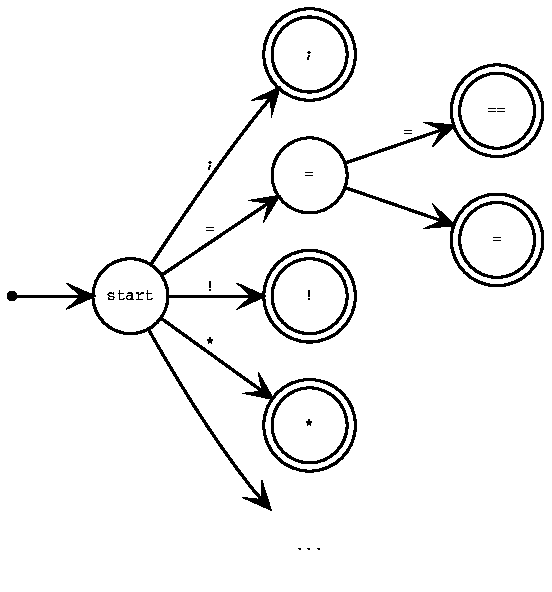
\includegraphics[scale=0.6]{{figures/figure02.04}.jpg}}
\end{center}
\end{frame}

\begin{frame}[fragile]
\pause

\begin{lstlisting}[language=Java]
switch (ch) {
...
case ';':
    nextCh();             
    return new TokenInfo(SEMI, line);         
case '=':             
    nextCh();             
    if (ch == '=') {                 
        nextCh();                 
        return new TokenInfo(EQUAL, line);             
    }             
    else {                 
        return new TokenInfo(ASSIGN, line);             
    }         
case '!':             
    nextCh();             
    return new TokenInfo(LNOT, line);         
case '*':             
    nextCh();             
    return new TokenInfo(STAR, line);
...
}
\end{lstlisting}
\end{frame}

\begin{frame}[fragile]
\pause

A state transition diagram for whitespace and the corresponding code
\begin{center}
\visible<2->{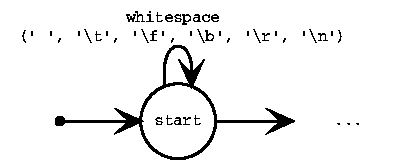
\includegraphics[scale=0.6]{{figures/figure02.05}.jpg}}
\end{center}

\begin{lstlisting}[language=Java]
while (isWhitespace(ch)) {                 
    nextCh();             
}
\end{lstlisting}
\end{frame}

\begin{frame}[fragile]
\pause

A state transition diagram for comments and the corresponding code
\begin{center}
\visible<2->{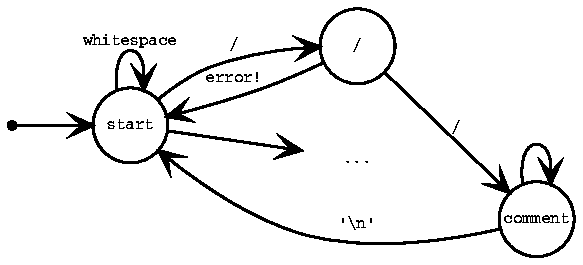
\includegraphics[scale=0.6]{{figures/figure02.06}.jpg}}
\end{center}
\end{frame}

\begin{frame}[fragile]
\pause

\begin{lstlisting}[language=Java]
boolean moreWhiteSpace = true;
while (moreWhiteSpace) {
    while (isWhitespace(ch)) {
        nextCh();
    }
    if (ch == '/') {
        nextCh();
        if (ch == '/') { 
            // CharReader maps all new lines to '\n'
            while (ch != '\n' && ch != EOFCH) {
                nextCh();
            }
        }
        else {
            reportScannerError("Operator / is not supported in j--.");
        }
    }
    else {
        moreWhiteSpace = false;
    }
}
\end{lstlisting}
\end{frame}

\section{Regular Expresssions}
\begin{frame}[fragile]
\pause

Regular expressions provide a simple notation for describing patterns of characters in a text

\pause
\bigskip

A regular expression defines a language of strings over an alphabet, and may take one of the following forms
\begin{enumerate}
\item If $a$ is in our alphabet, then the regular expression $a$ describes the language $L(a)$ consisting of the string $a$

\item If $r$ and $s$ are regular expressions then their concatenation $rs$ is also a regular expression describing the language $L(rs)$ of all possible strings obtained by concatenating a string in the language described by $r$, to a string in the language described by $s$

\item If $r$ and $s$ are regular expressions then the alternation $r|s$ is also a regular expression describing the language $L(r|s)$ consisting of all strings described by either $r$ or $s$

\item If $r$ is a regular expression, the repetition (aka the Kleene closure) $r*$ is also a regular expression describing the language $L(r*)$ consisting of strings obtained by concatenating zero or more instances of strings described by $r$ together

\item $\epsilon$ is a regular expression describing the language containing only the empty string

\item If $r$ is a regular expression, then $(r)$ is also a regular expression denoting the same language
\end{enumerate}
\end{frame}

\begin{frame}[fragile]
\pause

For example, given an alphabet $\{a,b\}$

\begin{enumerate}
\item $a(a|b)*$ denotes the language of non-empty strings of $a$'s and $b$'s, beginning with an $a$
\item $aa | ab | ba | bb$ denotes the language of all two-symbol strings over the alphabet
\item $(a|b)\!*\!ab$ denotes the language of all strings of $a$'s and $b$'s, ending in $ab$
\end{enumerate}

\pause
\bigskip

As another example, in a programming language such as Java
\begin{enumerate}
\item Reserved words may be described as \lstinline{abstract | boolean | char | ... | while}

\item Operators may be described as \lstinline{= | == | > | ... | *}

\item Identifiers may be described as \lstinline{([a-zA-Z] | _ | $)([a-zA-Z0-9] | _ | $)*}
\end{enumerate}
\end{frame}

\section{Finite State Automata}
\begin{frame}[fragile]
\pause

For any language described by a regular expression, there is a state transition diagram called Finite State Automaton that can parse strings in the language

\pause
\bigskip

A Finite State Automaton (FSA) $F$ is a quintuple $F = (\Sigma, S, s_0, M, F)$ where
\begin{itemize}
\item $\Sigma$ is the input alphabet
\item $S$ is a set of states
\item $s_0 \in S$ is a special start state
\item $M$ is a set of moves or state transitions of the form $$m(r, a) = s \text{ where } r,s \in S, a \in \Sigma$$ read as, ``if one is in state $r$, and the next input symbol is $a$, scan the $a$ and move into state $s$
\item $F \in S$ is a set of final states
\end{itemize}
\end{frame}

\begin{frame}[fragile]
\pause

For example, consider the regular expression $(a|b)a\!*\!b$ over the alphabet $\{a, b\}$ that describes the language consisting of all strings starting with either an $a$ or a $b$, followed by zero or more $a$'s, and ending with a $b$

\pause
\bigskip

An FSA $F$ that recognizes the language is $F = (\Sigma, S, s_0, M, F)$ where $\Sigma = \{a, b\}, S = \{0, 1, 2\}, s_0 = 0, M = \{m(0, a) = 1, m(0, b) = 1, m(1, a) = 1, m(1, b) = 2\}, F = \{2\}$

\pause
\bigskip

The corresponding transition diagram is shown below
\begin{center}
\visible<4->{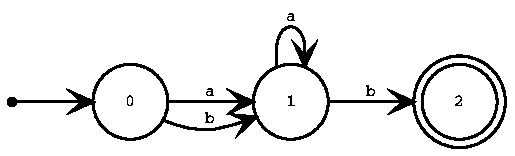
\includegraphics[scale=0.6]{{figures/figure02.07}.jpg}}
\end{center}
\end{frame}

\begin{frame}[fragile]
\pause

An FSA recognizes strings in the same way that state transition diagrams do 

\pause
\bigskip

For the previous FSA, given the input sentence $baaab$ and beginning in the start state 0, the following moves are prescribed

\begin{itemize}
\item $m(0, b)  = 1 \implies$ in state 0 we scan a $b$ and go into state 1
\item $m(1, a)  = 1 \implies$ in state 1 we scan an $a$ and go back into state 1
\item $m(1, a)  = 1 \implies$ in state 1 we scan an $a$ and go back into state 1 (again)
\item $m(1, a)  = 1 \implies$ in state 1 we scan an $a$ and go back into state 1 (again)
\item $m(1, b)  = 2 \implies$ finally, in state 1 we scan a $b$ and go into the final state 2
\end{itemize}

\begin{center}
\visible<3->{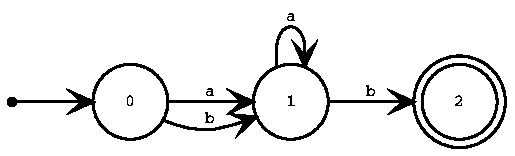
\includegraphics[scale=0.6]{{figures/figure02.07}.jpg}}
\end{center}
\end{frame}


\section{Non-deterministic (NFA) Versus Deterministic Finite State Automata (DFA)}
\begin{frame}[fragile]
\pause

A deterministic finite state automaton (DFA) is an automaton without $\epsilon$-moves, and there is a unique move from any state on an input symbol $a$, ie, there cannot be two moves $m(r, a) = s$ and $m(r, a) = t$, \noindent where $s \neq t$

\pause
\bigskip

A non-deterministic finite state automaton (NFA) is an automaton that allows either of the following
\begin{itemize}
\item More than one move from the same state, on the same input symbol $a$, ie, $m(r, a) = s$ and $m(r, a) = t$, \noindent where $s \neq t$

\item An $\epsilon$-move defined on the empty string $\epsilon$, ie, $m(r, \epsilon) = s$, which says we can move from state $r$ to state $s$ without scanning any input symbols
\end{itemize}
\end{frame}

\begin{frame}[fragile]
\pause

For example, an NFA that recognizes all strings of $a$'s and $b$'s that begin with an $a$ and end with a $b$ is $N = (\Sigma, S, s_0, M, F)$ where $\Sigma = \{a, b\}$, $S = \{0, 1, 2\}$, $s_0 = 0$, $M =  \{m(0, a) = 1, m(1, a) = 1, m(1, b) = 1, m(1, \epsilon) = 0, m(1, b) = 2\}$ and, $F = \{2\}$

\pause
\bigskip

The corresponding transition diagram is shown below
\begin{center}
\visible<3->{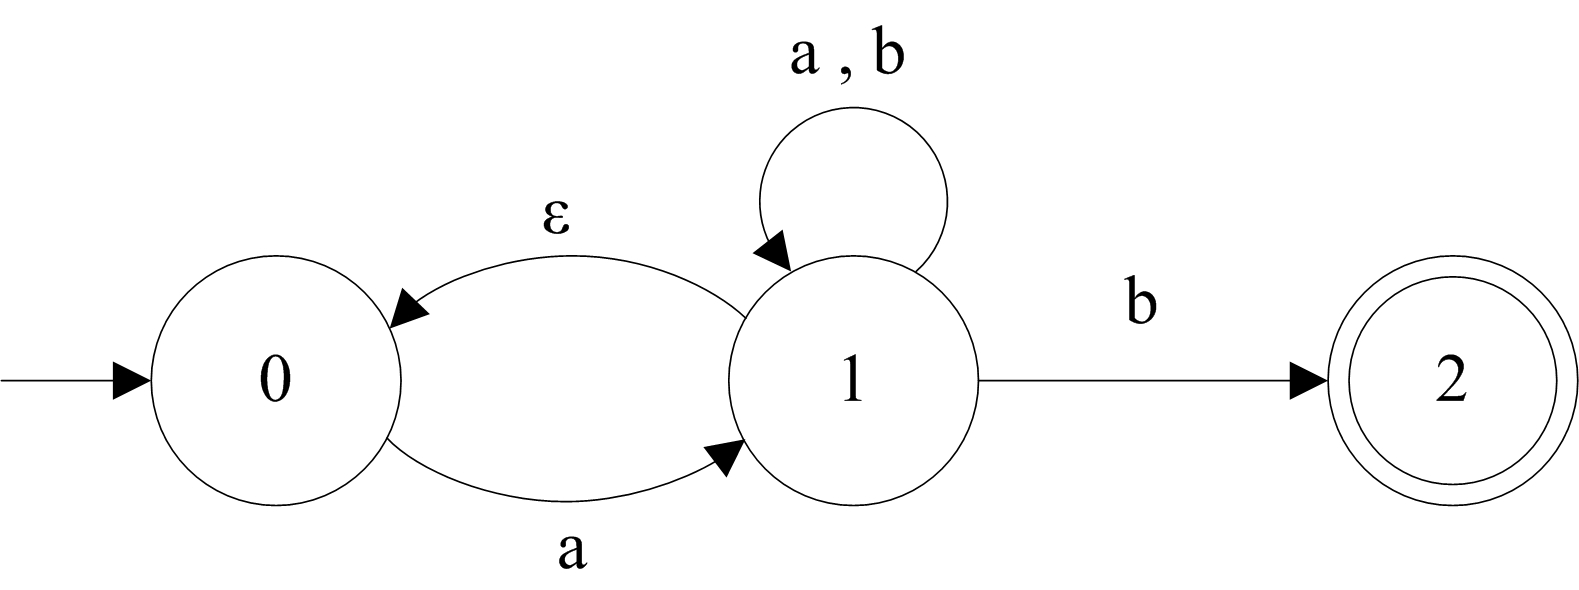
\includegraphics[scale=0.6]{{figures/figure02.08}.jpg}}
\end{center}

\pause
\bigskip

An NFA is said to recognize an input string if, starting in the start state, there exists a set of moves based on the input that takes us into one of the final states
\end{frame}

\section{Regular Expresssions to NFA}
\begin{frame}[fragile]
\pause

Given any regular expression $r$, we can construct (using Thompson's construction procedure) an NFA $N$ that recognizes the same language; ie, $L(N) = L(r)$

\pause
\bigskip

(Rule 1) If the regular expression $r$ takes the form of an input symbol, $a$, then the NFA that recognizes it has two states: a start state and a final state, and a move on symbol $a$ from the start state to the final state

\begin{center}
\visible<3->{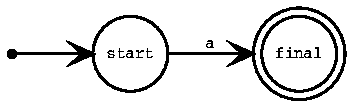
\includegraphics[scale=0.6]{{figures/figure02.09}.jpg}}
\end{center}

\pause
\bigskip

(Rule 2) If $N_r$ and $N_s$ are NFA recognizing the languages described by the regular expressions $r$ and $s$ respectively, then we can create a new NFA recognizing the language described by $rs$ as follows: we define an $\epsilon$-move from the final state of $N_r$  to the start state of $N_s$, then choose the start state of $N_r$ to be our new start state, and the final state of $N_s$ to be our new final state

\begin{center}
\visible<4->{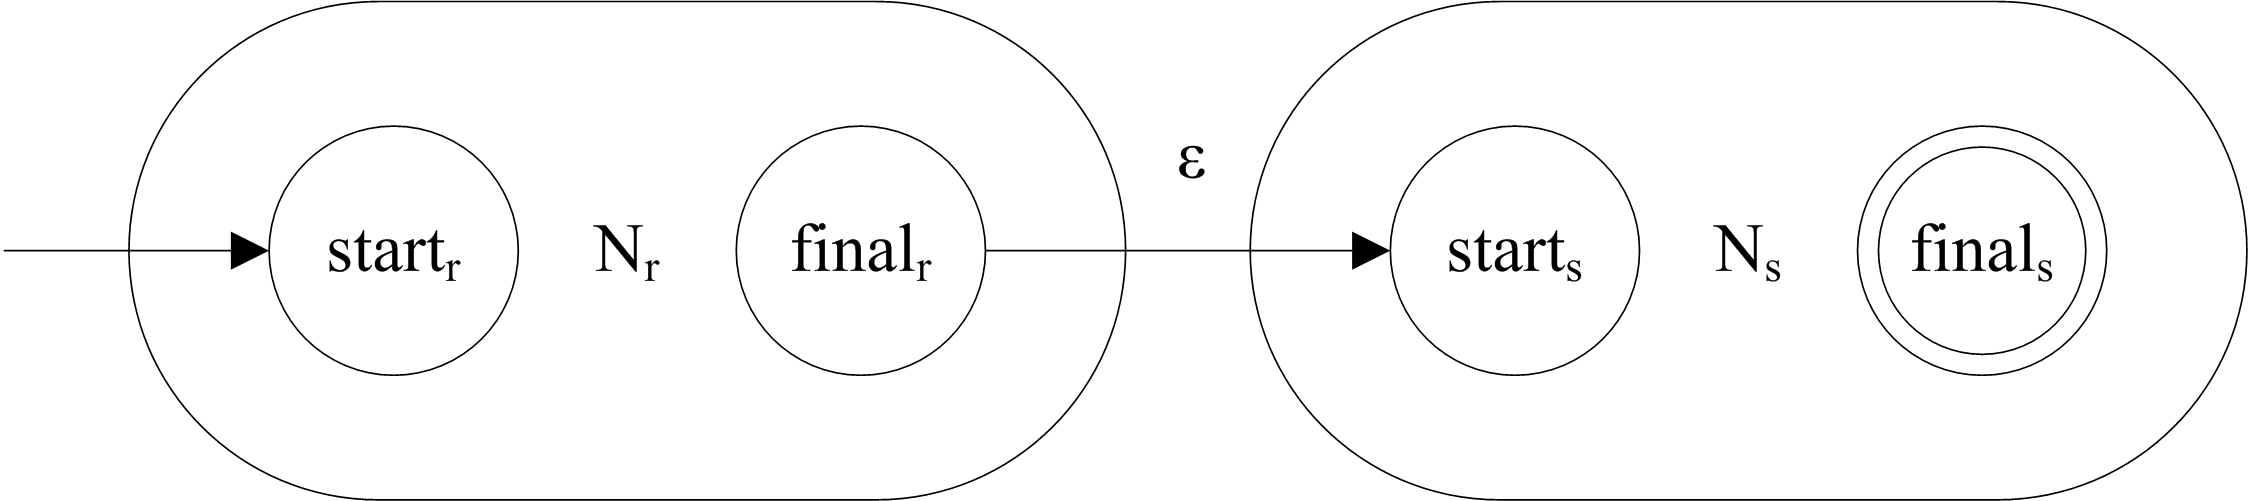
\includegraphics[scale=0.6]{{figures/figure02.10}.jpg}}
\end{center}
\end{frame}

\begin{frame}[fragile]
\pause

(Rule 3) If $N_r$ and $N_s$ are NFA recognizing the languages described by the regular expressions $r$ and $s$ respectively, then we can create a new NFA recognizing the language described by $r|s$ as follows: we define a new start state, having $\epsilon$-moves to each of the start states of $N_r$ and $N_s$, and we define a new final state and add $\epsilon$-moves from each of the final states of $N_r$ and $N_s$ to this state

\begin{center}
\visible<2->{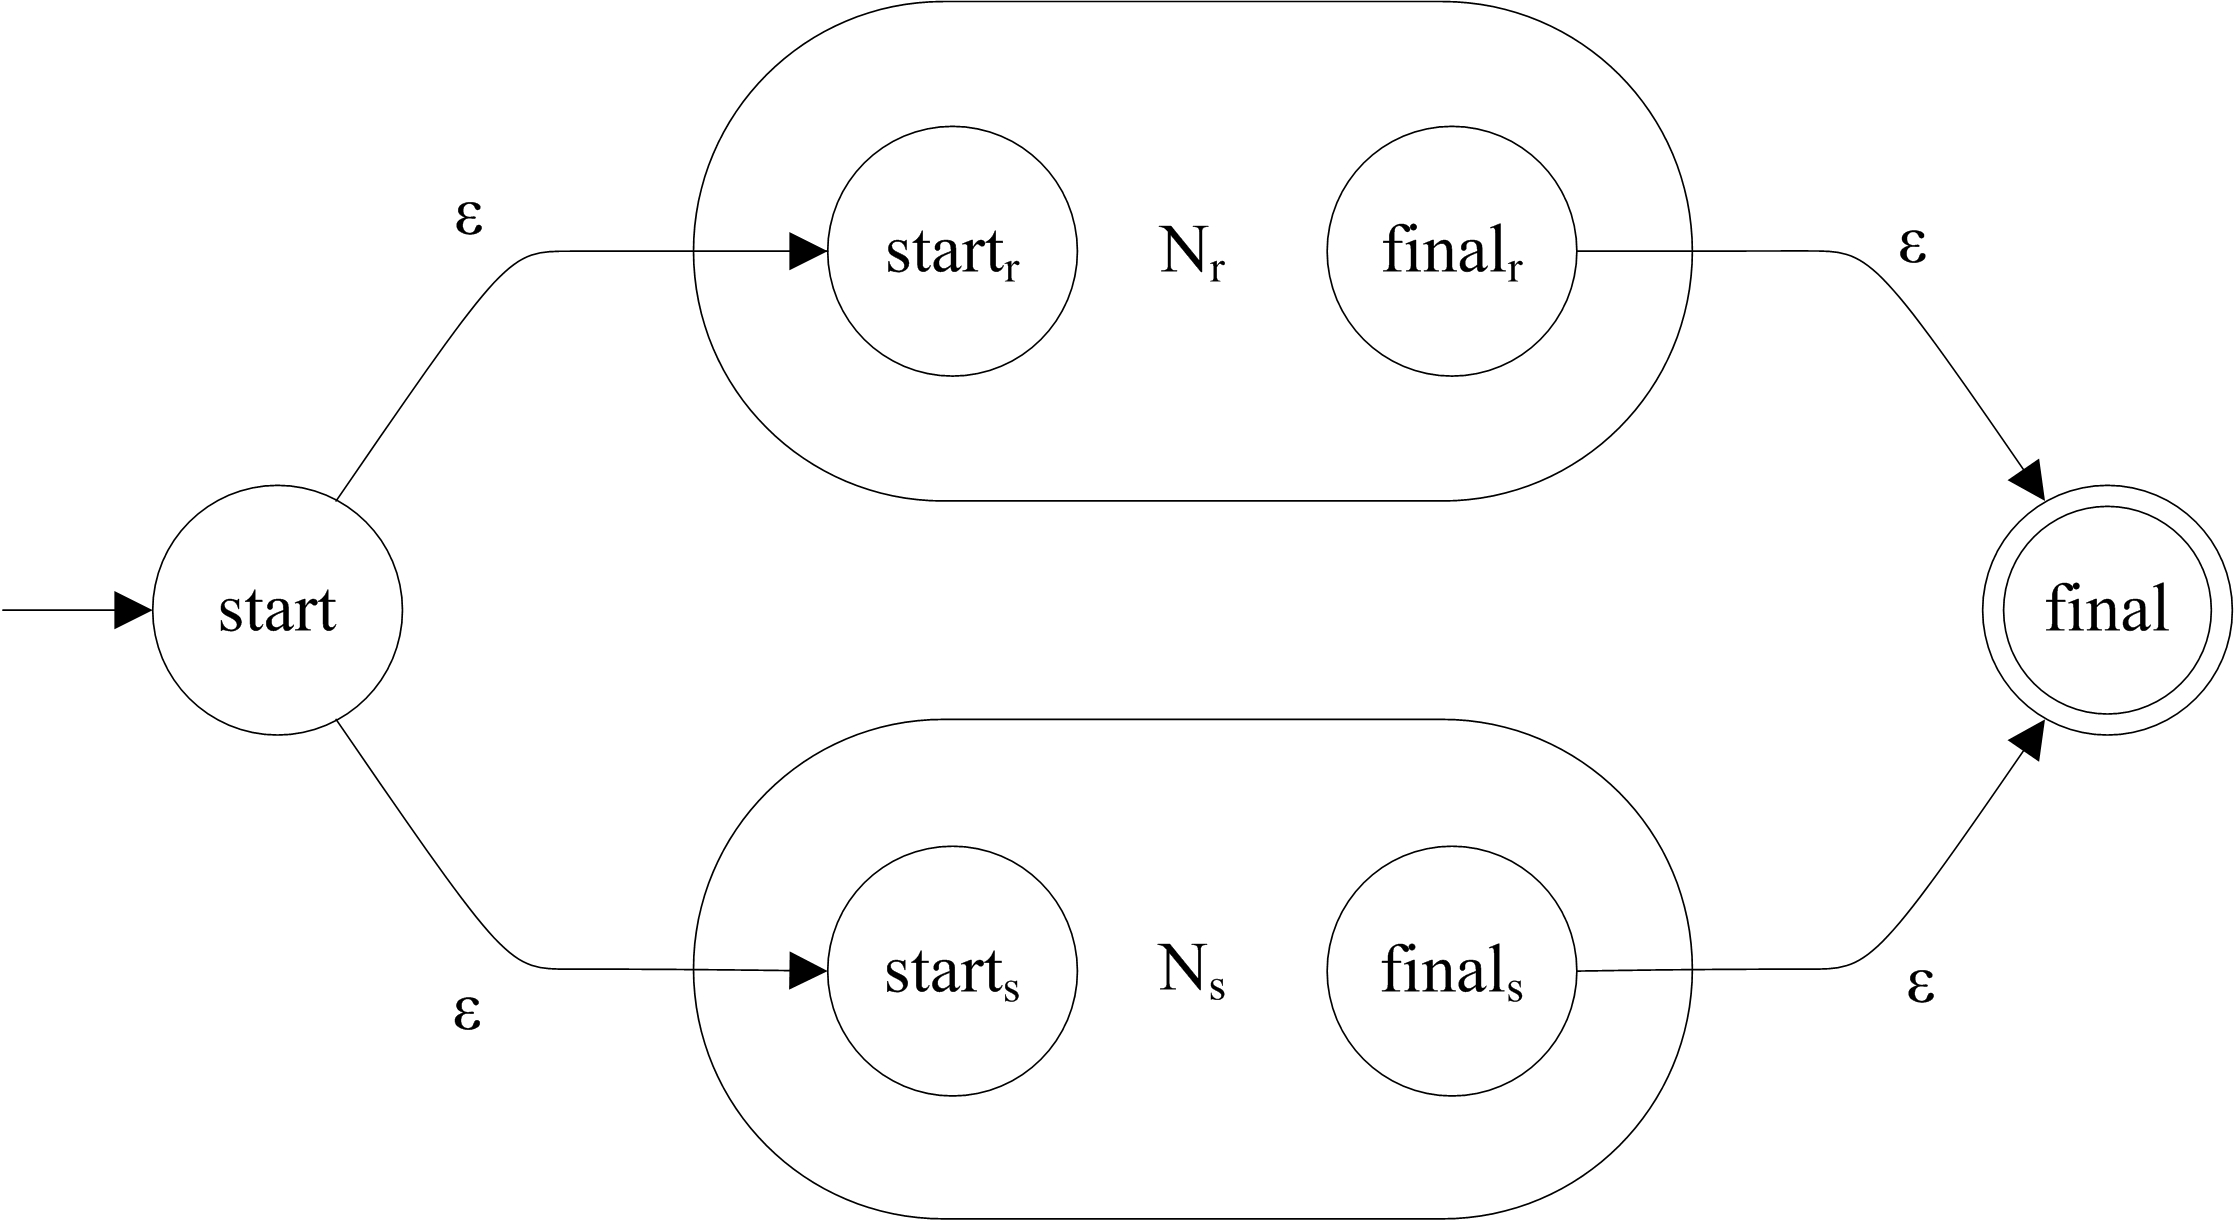
\includegraphics[scale=0.6]{{figures/figure02.11}.jpg}}
\end{center}
\end{frame}

\begin{frame}[fragile]
\pause

(Rule 4) If $N_r$ is an NFA recognizing that language described by a regular expression $r$, then we construct a new NFA recognizing $r*$ as follows:  we add an $\epsilon$-move from $N_r$'s final state back to its start state, define a new start state and a new final state, add $\epsilon$-moves from the new start state to both $N_r$'s start state and the new final state, and define an $\epsilon$-move from $N_r$'s final state to the new final state

\begin{center}
\visible<2->{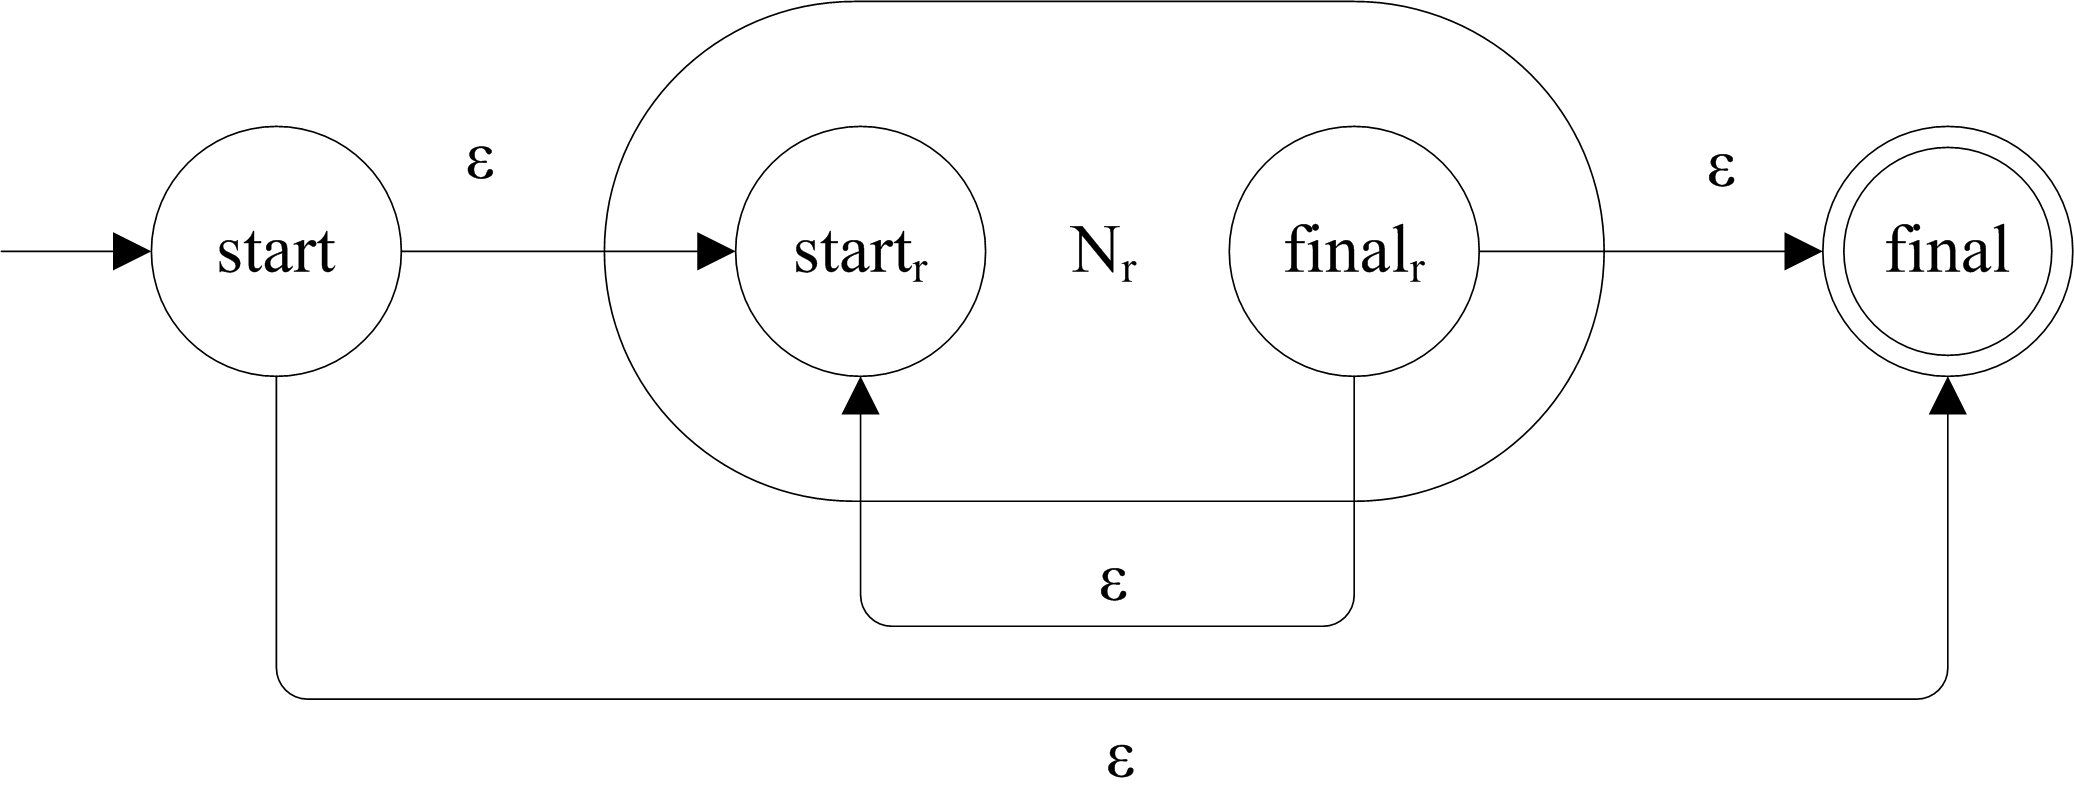
\includegraphics[scale=0.6]{{figures/figure02.12}.jpg}}
\end{center}

\pause
\bigskip

(Rule 5) If $r$ is $\epsilon$ then we just need an $\epsilon$-move from the start state to the final state

\begin{center}
\visible<3->{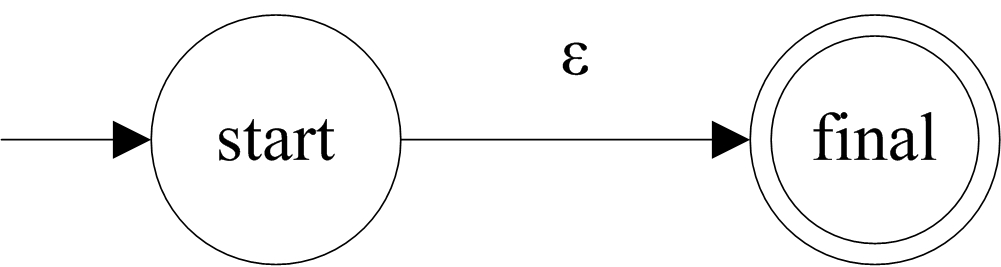
\includegraphics[scale=0.6]{{figures/figure02.13}.jpg}}
\end{center}

\pause
\bigskip

(Rule 6) If $N_r$ is our NFA recognizing the language described by $r$, then $N_r$ also recognizes the language described by $(r)$
\end{frame}

\begin{frame}[fragile]
\pause

As an example, let's construct an NFA for the regular expression $(a|b)a\!*\!b$, which has the following syntactic structure

\begin{center}
\visible<2->{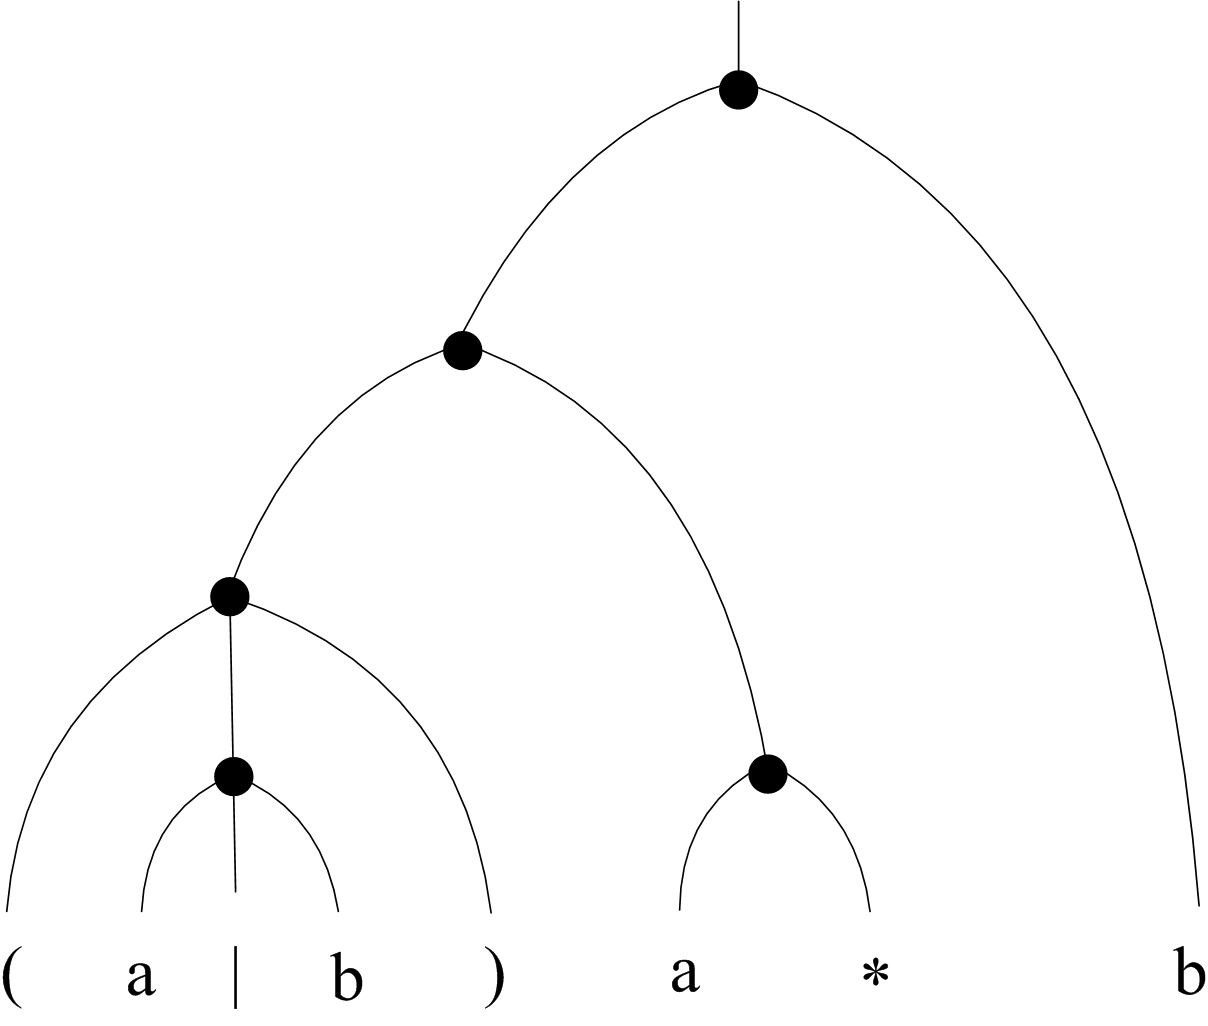
\includegraphics[scale=0.6]{{figures/figure02.14}.jpg}}
\end{center}

\pause
\bigskip

We start with the first $a$ and $b$; the automata recognizing these are easy enough to construct using Rule 1

\begin{center}
\visible<3->{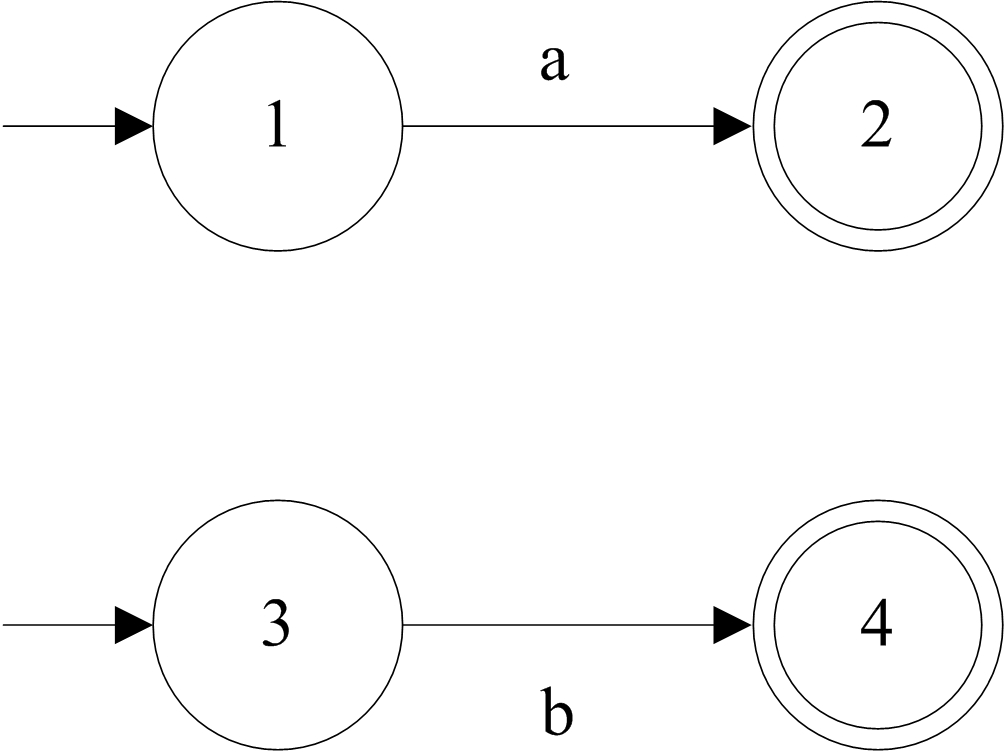
\includegraphics[scale=0.6]{{figures/construction-a1}.jpg}}
\end{center}
\end{frame}

\begin{frame}[fragile]
\pause

We then put them together using Rule 3 to produce an NFA recognizing $a|b$

\begin{center}
\visible<2->{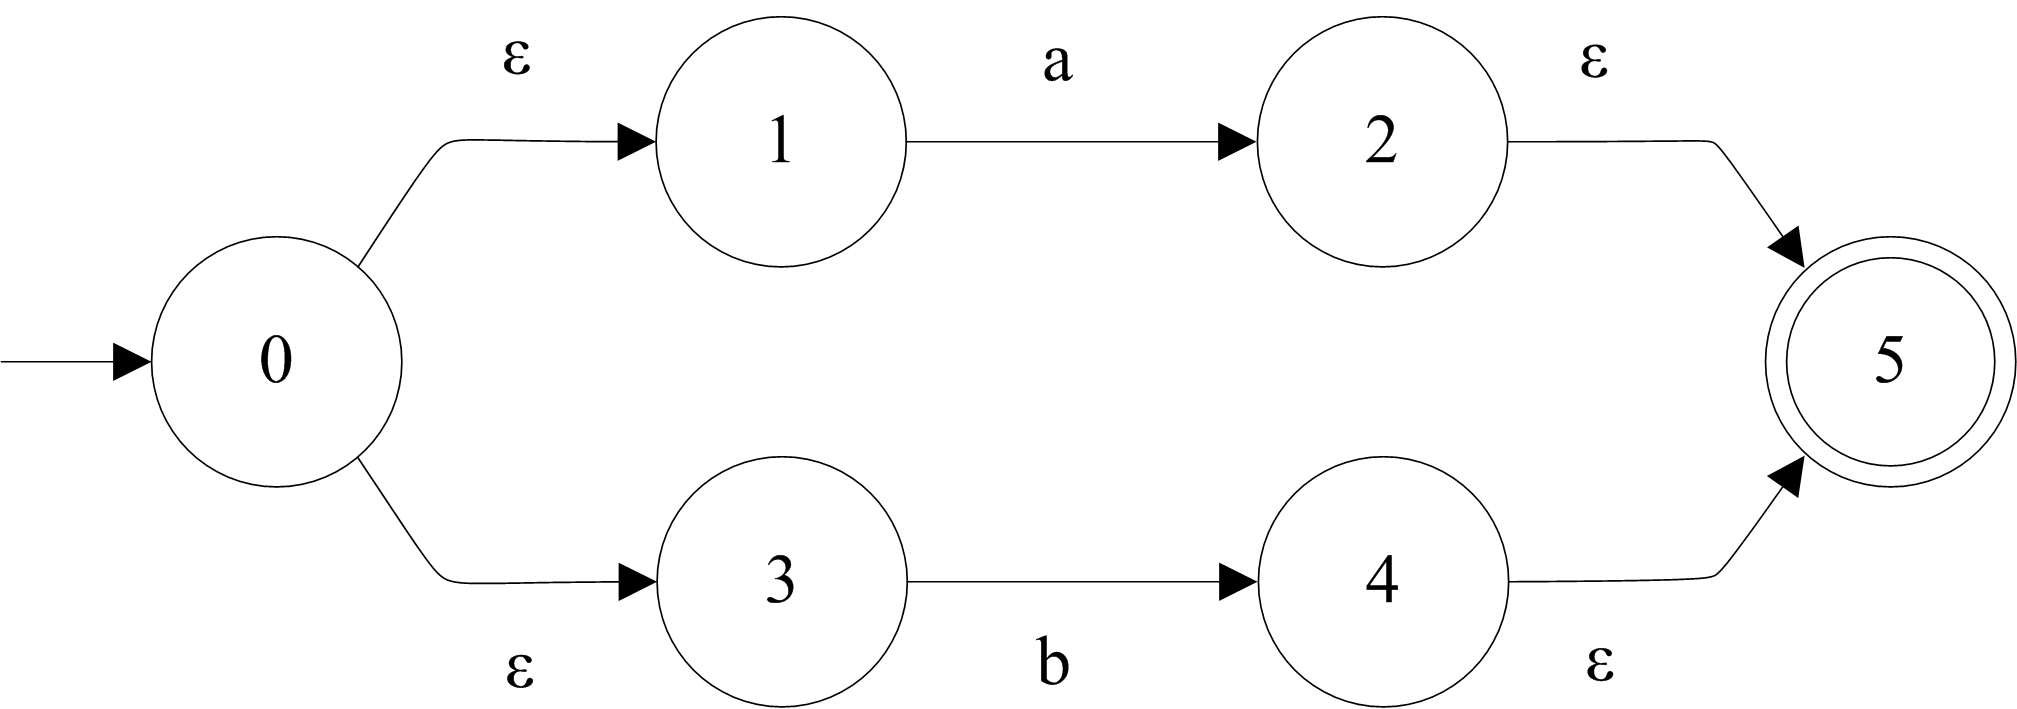
\includegraphics[scale=0.6]{{figures/construction-a2}.jpg}}
\end{center}

\pause
\bigskip

The NFA recognizing $(a|b)$ is the same as that recognizing $a|b$, by Rule 6

\pause
\bigskip

An NFA recognizing the second instance of $a$ is simple enough, by Rule 1 again

\begin{center}
\visible<4->{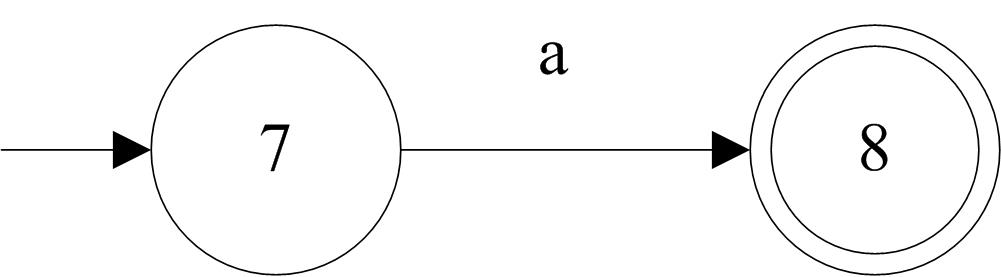
\includegraphics[scale=0.6]{{figures/construction-a3}.jpg}}
\end{center}

\pause
\bigskip

The NFA recognizing $a*$ can be constructed from the NFA for $a$, by applying Rule 4

\begin{center}
\visible<5->{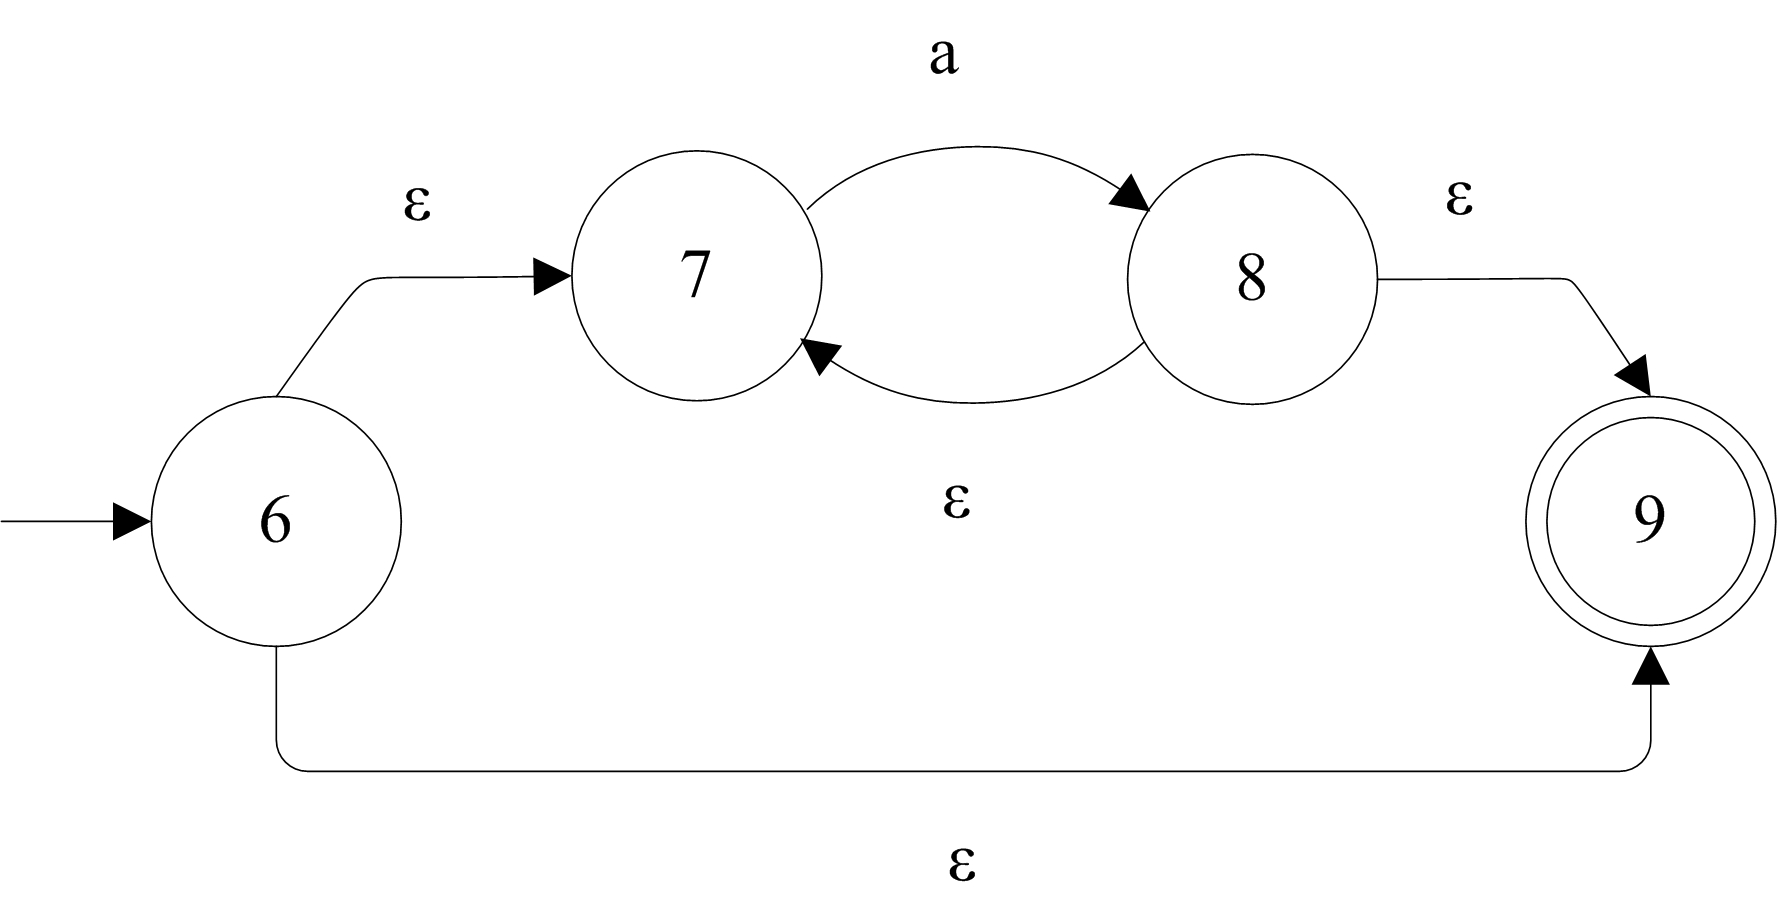
\includegraphics[scale=0.6]{{figures/construction-a4}.jpg}}
\end{center}
\end{frame}

\begin{frame}[fragile]
\pause

We then apply Rule 2 to construct an NFA recognizing the concatenation $(a|b)a*$

\begin{center}
\visible<2->{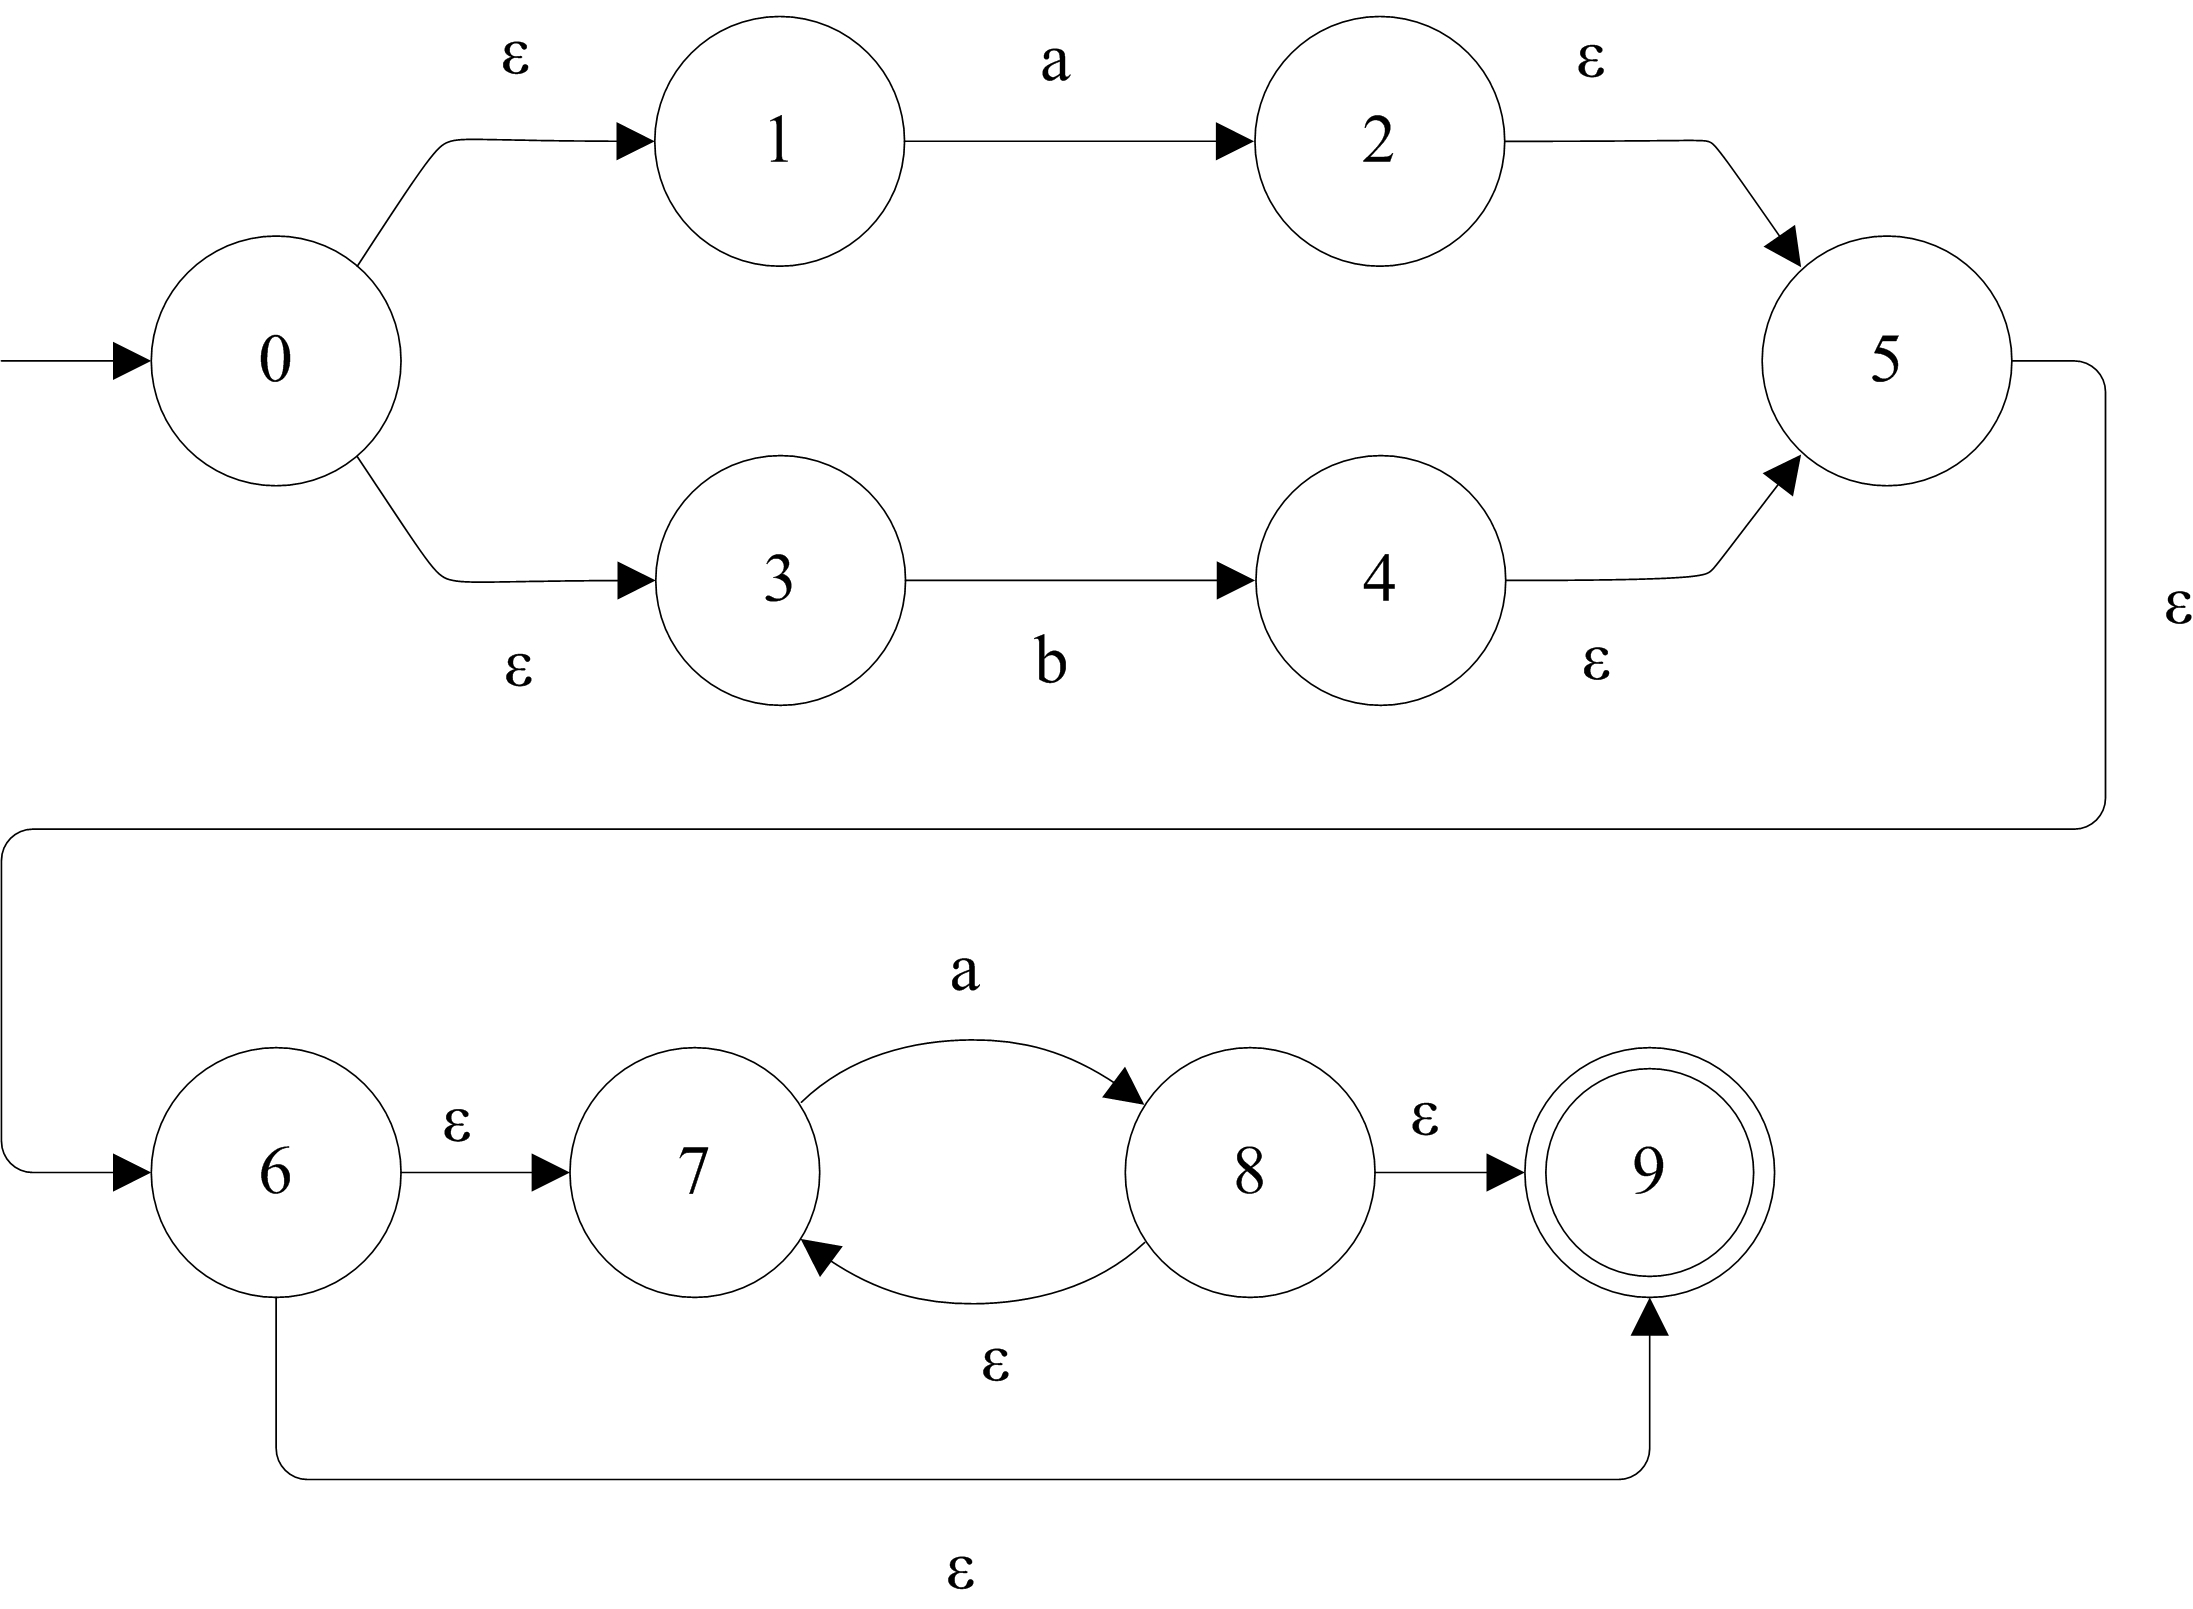
\includegraphics[scale=0.6]{{figures/construction-a5}.jpg}}
\end{center}
\end{frame}

\begin{frame}[fragile]
\pause

An NFA recognizing the second instance of $b$ is simple enough, by Rule 1 again

\begin{center}
\visible<2->{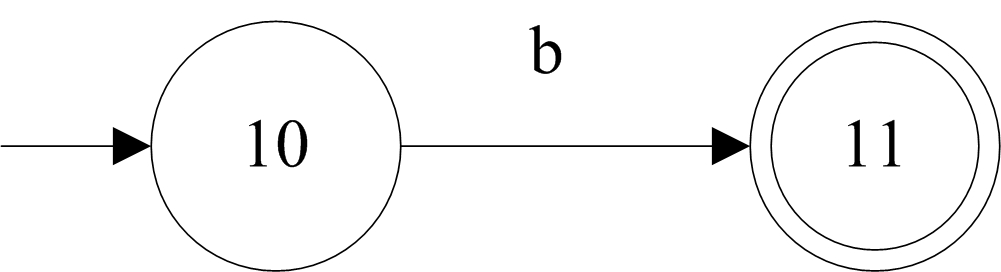
\includegraphics[scale=0.6]{{figures/construction-a6}.jpg}}
\end{center}

\pause
\bigskip

Finally, we can apply Rule 2 again to produce an NFA recognizing $(a|b)a\!*\!b$

\begin{center}
\visible<3->{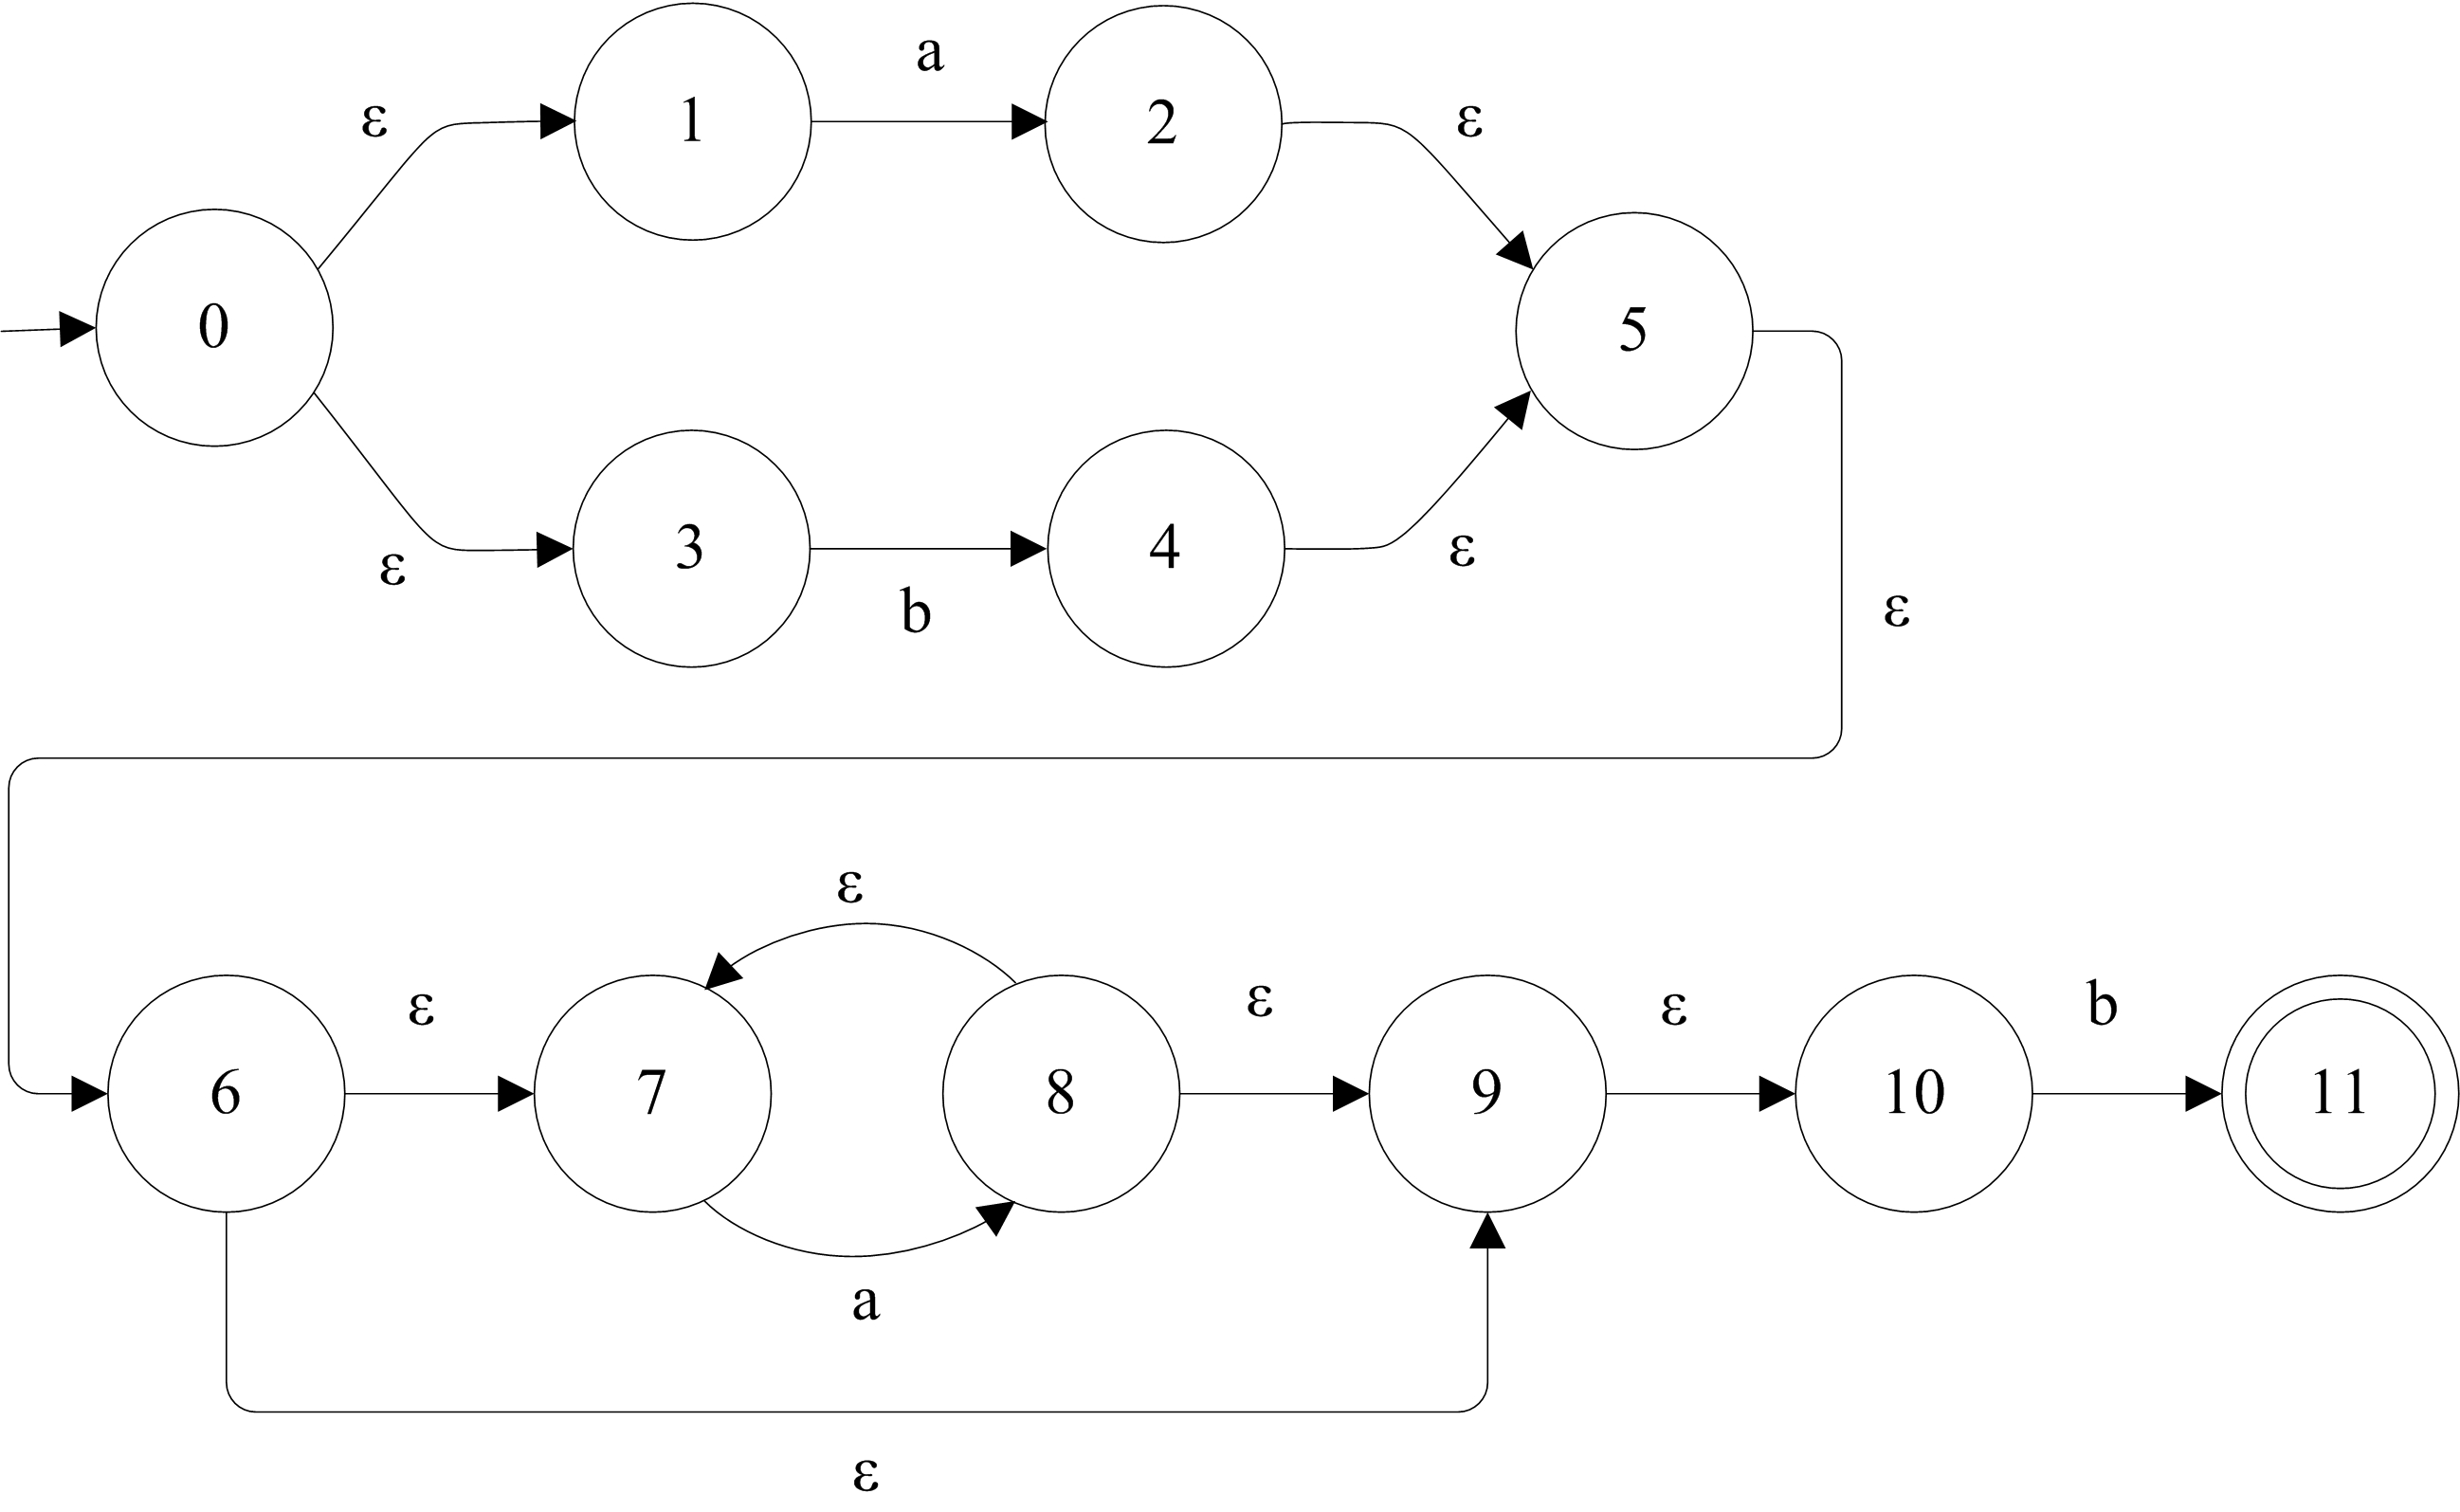
\includegraphics[scale=0.6]{{figures/figure02.15}.jpg}}
\end{center}
\end{frame}

\section{NFA to DFA}
\begin{frame}[fragile]
\pause

\end{frame}

\section{A Minimal DFA}
\begin{frame}[fragile]
\pause

\end{frame}

\section{JavaCC: a Tool for Generating Scanners}
\begin{frame}[fragile]
\pause

\end{frame}
\end{document}
